\documentclass[11pt]{article}
\usepackage{notesstyle}

\begin{document}
\notesheader{3.11}{Working with Time Series}{Timestamps, periods, and durations --- and the indexing, resampling, and rolling machinery built on top of them.}

\section{Why time deserves its own machinery}

\begin{background}
Time is the one ``label'' almost every real dataset carries: a sensor reading, a stock tick, a server log line, a patient visit. You could in principle store dates as plain strings and reason about them by hand --- but the moment you want to ask ``give me every row in July 2021,'' ``average this by month,'' or ``smooth this over a 30-day window,'' string handling collapses. You need an index that \emph{understands} that 2021-07-31 is followed by 2021-08-01, that a month is not a fixed number of days, and that subtracting two dates yields a \emph{duration}.

Python's story here is a layered one, and it helps to know the layers because Pandas stitches them together:
\begin{itemize}
  \item \textbf{The standard library: \code{datetime} (and \code{dateutil}).} Python ships a \code{datetime} type, and the third-party \code{dateutil} adds flexible parsing (``\code{4th of July, 2021}'' just works). This stack is wonderfully flexible but \emph{slow}: each date is a full Python object, so a column of a million dates is a million-pointer object array.
  \item \textbf{NumPy's \code{datetime64}.} NumPy encodes a date as a 64-bit integer (a count of time units from a fixed epoch). This is fast, typed, and vectorizes like any other NumPy array --- but it is \emph{rigid}: one fixed unit per array, and none of the friendly parsing or calendar logic.
\end{itemize}
\textbf{Pandas unifies the two.} It gives you a \code{Timestamp} object that has the \emph{convenience} of \code{datetime} but is built on the \emph{speed} of \code{datetime64}, and --- crucially --- a \code{DatetimeIndex} that turns an axis of timestamps into a first-class, sliceable, groupable index.
\end{background}

\begin{lstlisting}
import numpy as np
import pandas as pd
\end{lstlisting}

\begin{pyrefresh}
A 64-bit integer counting fixed-size units from an \emph{epoch} (the reference instant \code{1970-01-01T00:00:00}) is exactly how Unix ``epoch time'' works. \code{datetime64} generalizes it: the same integer can count \emph{nanoseconds}, \emph{days}, \emph{years}, etc. The unit is part of the dtype, written like \code{datetime64[ns]} (nanoseconds) or \code{datetime64[D]} (days). Pandas standardizes on nanosecond resolution.
\end{pyrefresh}

\section{The three kinds of time data}

Before any API, fix the vocabulary. There are three conceptually distinct things you might mean by ``a time,'' and Pandas gives each its own scalar type \emph{and} its own index type.

\begin{center}
\renewcommand{\arraystretch}{1.3}
\begin{tabular}{l l l l}
\toprule
\textbf{Concept} & \textbf{Meaning} & \textbf{Scalar class} & \textbf{Index class} \\
\midrule
Time \emph{stamp}    & a single instant (a point)        & \code{Timestamp} & \code{DatetimeIndex} \\
Time \emph{period}   & a fixed-frequency interval (a bin) & \code{Period}    & \code{PeriodIndex} \\
Time \emph{duration} & an elapsed span (a length)        & \code{Timedelta} & \code{TimedeltaIndex} \\
\bottomrule
\end{tabular}
\end{center}

\begin{intuition}
The cleanest way to keep these straight is geometric --- think of a timeline:
\begin{itemize}
  \item A \textbf{timestamp} is a \emph{point} on the line: ``3:00\,pm on July 4th.''
  \item A \textbf{period} is a \emph{labeled interval} of fixed frequency: ``the month of July 2021'' --- it has an anchor and a width, and consecutive periods tile the line without gaps.
  \item A \textbf{duration} is a \emph{length} with no fixed position: ``90 minutes.'' Subtract two timestamps and you get one.
\end{itemize}
\end{intuition}

\begin{center}
\begin{tikzpicture}[font=\sffamily\small,
    >=Stealth, every node/.style={font=\sffamily\footnotesize}]
  % the timeline axis
  \draw[->, thick, accent] (0,0) -- (12,0) node[right, accent]{time};
  \foreach \x/\lab in {1/Jun, 4/Jul, 7/Aug, 10/Sep} {
    \draw[accent] (\x,0.12) -- (\x,-0.12);
    \node[below=2pt, color=accent] at (\x,-0.12) {\lab\,1};
  }

  % TIMESTAMP: a point
  \filldraw[purpleaccent] (5,0) circle (2.6pt);
  \node[purpleaccent, above=4pt] at (5,0) {\textbf{timestamp}};
  \node[purpleaccent, above=16pt] at (5,0) {a \emph{point}};

  % PERIOD: a shaded interval (the July bin)
  \begin{scope}[on background layer]
    \fill[bggreen] (4,-0.7) rectangle (7,-0.05);
  \end{scope}
  \draw[accent2, thick] (4,-0.7) rectangle (7,-0.05);
  \node[accent2, below=2pt] at (5.5,-0.7) {\textbf{period} ``Jul 2021'' --- a \emph{bin}};

  % DURATION: a span between two points, drawn above
  \filldraw[warn] (8.5,1.0) circle (2pt);
  \filldraw[warn] (11,1.0) circle (2pt);
  \draw[warn, thick, <->] (8.5,1.0) -- (11,1.0)
        node[midway, above, warn]{\textbf{duration}};
  \node[warn, below=1pt] at (9.75,1.0) {a \emph{length}};
\end{tikzpicture}
\end{center}

\subsection{Creating each, by hand}

\begin{lstlisting}
ts = pd.Timestamp('2021-07-04 15:00')   # a point in time
pr = pd.Period('2021-07', freq='M')     # the whole month of July 2021
td = pd.Timedelta(days=90)              # a 90-day length

ts2 = pd.Timestamp('2021-10-02 15:00')
ts2 - ts                                # subtracting points -> a Timedelta
\end{lstlisting}

\begin{outbox}
Timedelta('90 days 00:00:00')
\end{outbox}

Note the arithmetic that ties them together: \code{Timestamp} $-$ \code{Timestamp} $=$ \code{Timedelta}, and \code{Timestamp} $+$ \code{Timedelta} $=$ \code{Timestamp}. Periods behave like calendar bins: \code{pr + 1} is August 2021, and \code{ts in pr} tests whether the instant falls inside the bin.

\subsection{Converting between the three}

These types are not islands; you move between them constantly, and knowing the conversions saves a lot of fumbling:
\begin{itemize}
  \item \textbf{Stamp $\to$ period} with \code{.to\_period(freq)}: ``which bin does this instant fall in?'' A \code{DatetimeIndex} of daily readings becomes a \code{PeriodIndex} of months via \code{idx.to\_period('M')} --- handy right before a group-by-month.
  \item \textbf{Period $\to$ stamp} with \code{.to\_timestamp(how=...)}: collapse a bin back to a point, anchoring at its \code{'start'} or \code{'end'}.
  \item \textbf{Stamp $\to$ duration} by subtraction, as above; and a \code{DatetimeIndex} minus a single \code{Timestamp} yields a \code{TimedeltaIndex} of elapsed times --- the natural ``time since launch'' axis.
\end{itemize}

\begin{lstlisting}
p = pd.Timestamp('2021-07-04 15:00').to_period('M')  # Period('2021-07','M')
p.to_timestamp(how='start')   # -> Timestamp('2021-07-01 00:00:00')
p.to_timestamp(how='end')     # -> Timestamp('2021-07-31 23:59:59.999...')
\end{lstlisting}

Notice the asymmetry: a stamp carries \emph{more} information than the period it maps to (the exact instant), so \code{to\_period} \emph{discards} detail, while \code{to\_timestamp} has to \emph{invent} a convention (start vs.\ end) to recover a point. Conversions that lose information are one-way --- a recurring theme worth flagging to yourself whenever you reach for one.

\section{Constructors: building indexes in bulk}

You rarely create one timestamp at a time. The workhorses are \code{pd.to\_datetime} (parse whatever you have into timestamps) and the \code{*\_range} family (manufacture a regular grid).

\subsection{Parsing: \texttt{pd.to\_datetime}}

\code{pd.to\_datetime} is the flexible front door. Hand it a single string and you get a \code{Timestamp}; hand it a list/array/column and you get a \code{DatetimeIndex}. It understands a remarkable range of formats:

\begin{lstlisting}
pd.to_datetime('4th of July, 2021')     # -> Timestamp('2021-07-04 00:00:00')
dates = pd.to_datetime(['2021-07-04', '2021-07-05', '2021-07-08'])
print(dates)
\end{lstlisting}

\begin{outblock}
DatetimeIndex(['2021-07-04', '2021-07-05', '2021-07-08'],
              dtype='datetime64[ns]', freq=None)
\end{outblock}

\begin{pitfall}
\textbf{Day-first vs. month-first ambiguity.} A string like \code{'04/07/2021'} is genuinely ambiguous: is it April 7th or July 4th? \code{to\_datetime} defaults to \emph{month-first} (US style) and will silently pick July\,\dots\,sorry, \emph{April}. If your data is day-first, pass \code{dayfirst=True}. Better still, when you know the exact layout, pass an explicit \code{format='\%d/\%m/\%Y'}: it is both unambiguous \emph{and} much faster, because it skips the format-sniffing step on every value.
\end{pitfall}

\subsection{Regular grids: the \texttt{*\_range} family}

To manufacture a regular sequence, choose the constructor that matches the \emph{kind} of data you want:

\begin{lstlisting}
pd.date_range('2021-07-01', periods=5, freq='D')      # 5 daily timestamps
pd.date_range('2021-07-01', '2021-07-10', freq='2D')  # every 2nd day, by endpoints
pd.period_range('2021-01', periods=4, freq='M')       # 4 monthly periods
pd.timedelta_range(0, periods=4, freq='6H')           # 0h, 6h, 12h, 18h
\end{lstlisting}

\begin{outblock}
PeriodIndex(['2021-01', '2021-02', '2021-03', '2021-04'],
            dtype='period[M]')
\end{outblock}

You specify a range two ways: \code{start} $+$ \code{periods} (a count), or \code{start} $+$ \code{end} (by endpoints). The \code{freq} argument controls the spacing, and it is worth memorizing the common codes.

\subsection{Frequency and offset codes}

\begin{center}
\renewcommand{\arraystretch}{1.25}
\begin{tabular}{l l l l}
\toprule
\textbf{Code} & \textbf{Meaning} & \textbf{Code} & \textbf{Meaning} \\
\midrule
\code{D}  & calendar day            & \code{H}     & hour \\
\code{B}  & business day (Mon--Fri) & \code{T}/\code{min} & minute \\
\code{W}  & week (Sun-anchored)     & \code{S}     & second \\
\code{M}  & month \emph{end}        & \code{MS}    & month \emph{start} \\
\code{Q}  & quarter end             & \code{QS}    & quarter start \\
\code{A}/\code{Y} & year end          & \code{AS}/\code{YS} & year start \\
\bottomrule
\end{tabular}
\end{center}

\begin{keyidea}
Two patterns make the code list far more powerful than it looks:
\begin{itemize}
  \item \textbf{Numbers multiply.} Prefix a code with an integer to scale it: \code{'2D'} is every other day, \code{'3M'} is every third month-end.
  \item \textbf{Codes concatenate (add).} Stack codes to combine units: \code{'2H30T'} is a 2-hour-30-minute step, \code{'1D6H'} is 30 hours.
\end{itemize}
And mind the \code{S} suffix: a bare \code{M}, \code{Q}, \code{A} anchors to the \emph{end} of the period (so \code{date\_range(freq='M')} lands on Jan 31, Feb 28, \dots), while \code{MS}, \code{QS}, \code{YS} anchor to the \emph{start} (Jan 1, Feb 1, \dots). Picking the wrong one is a classic off-by-a-month bug in monthly reports.
\end{keyidea}

\section{Indexing by time}

The payoff for all this typing is that a \code{DatetimeIndex} makes time-based selection feel effortless. Put timestamps on the index of a \code{Series}, and you unlock \emph{partial-string indexing}.

\begin{lstlisting}
idx = pd.to_datetime(['2020-07-04', '2020-08-04',
                      '2021-07-04', '2021-08-04'])
data = pd.Series([0, 1, 2, 3], index=idx)
print(data)
\end{lstlisting}

\begin{outblock}
2020-07-04    0
2020-08-04    1
2021-07-04    2
2021-08-04    3
dtype: int64
\end{outblock}

Now you can select by a \emph{partial} date string, and Pandas interprets it as ``every timestamp that falls inside this calendar span'':

\begin{lstlisting}
data['2021']          # everything in the year 2021  -> the last two rows
data['2020-07']       # everything in July 2020       -> the first row
data['2020-08':'2021-07']   # an inclusive date-range slice
\end{lstlisting}

\begin{outbox}
2021-07-04 \quad 2 \\
2021-08-04 \quad 3 \\
dtype: int64
\end{outbox}

\begin{intuition}
Why does \code{data['2021']} return \emph{rows} when \code{df['col']} on a regular \code{DataFrame} returns a \emph{column}? Because a \code{DatetimeIndex} teaches the index how to ``parse'' a string into a span and match it against the row labels. \code{'2021'} is not a column name --- it is a coarse timestamp that resolves to the half-open interval $[\,$2021-01-01$,\,$2022-01-01$)$, and every label inside it comes back. This is the single most ergonomic feature of time-series Pandas.
\end{intuition}

\section{A worked synthetic series}

To make resampling and rolling concrete, we need a realistic daily series. We build one with a \emph{fixed seed} so the figures below are reproducible: a cumulative-sum random walk (the slow drift) plus a yearly sine term (the season) plus a little daily noise, indexed by a two-year \code{date\_range}.

\begin{lstlisting}
rng = np.random.default_rng(0)
dates = pd.date_range('2021-01-01', periods=730, freq='D')
seasonal = 8.0 * np.sin(2 * np.pi * dates.dayofyear / 365.0)
walk = np.cumsum(rng.normal(0.02, 1.0, size=len(dates)))  # the drift
noise = rng.normal(scale=1.5, size=len(dates))
series = pd.Series(50 + walk + seasonal + noise,
                   index=dates, name='signal')
\end{lstlisting}

\begin{figure}[h]
\centering
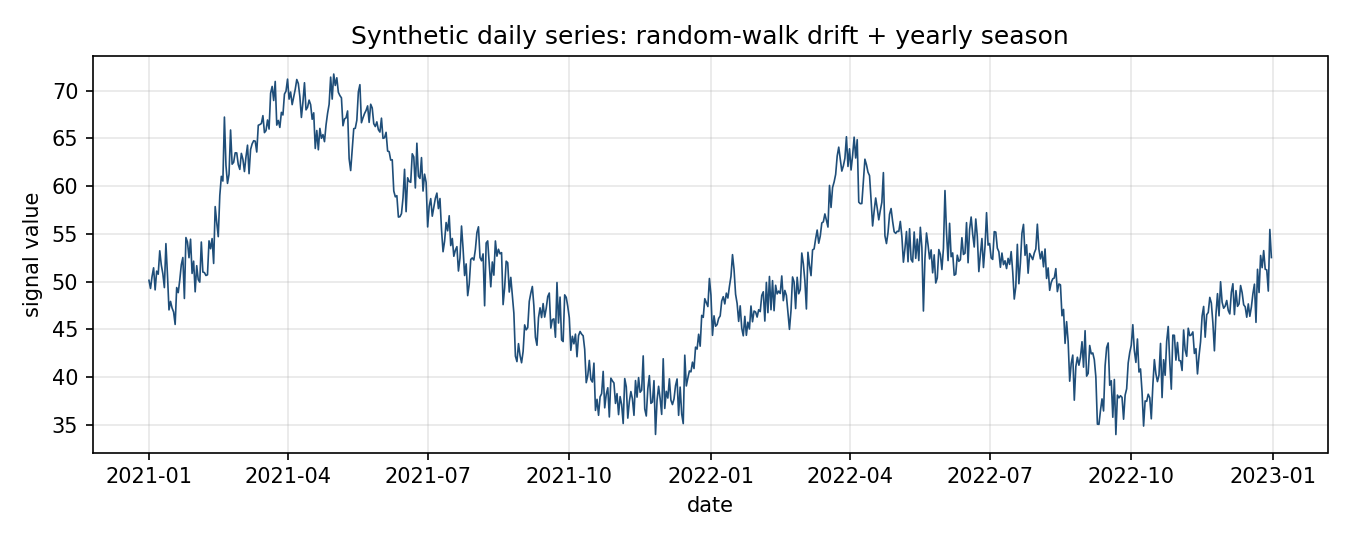
\includegraphics[width=\linewidth]{ts_raw.png}
\caption{The raw synthetic daily series. The slow up-and-down wander is the random-walk \emph{drift}; the gentle yearly bulge is the \emph{seasonal} sine term; the fuzz around the line is daily noise. Two years of daily data is 730 points --- dense enough that the underlying structure is hard to read by eye, which is exactly what motivates the smoothing tools below.}
\end{figure}

\section{Resampling and frequency conversion}

A daily series is often \emph{too} granular. Two distinct operations change its frequency, and conflating them is a common mistake.

\subsection{\texttt{resample}: a groupby over time bins}

\code{resample} is a \emph{reduction}. It chops the index into bins of the target frequency and applies an aggregation to each bin --- it is, almost literally, ``\code{groupby} where the grouping key is the time bin.''

\begin{lstlisting}
monthly = series.resample('M').mean()   # mean of each calendar month
monthly.head(3)
\end{lstlisting}

\begin{outblock}
2021-01-31    50.83
2021-02-28    52.11
2021-03-31    54.02
Freq: M, Name: signal, dtype: float64
\end{outblock}

Because it aggregates, \code{resample} naturally handles \textbf{down-sampling} (going to a \emph{coarser} frequency, e.g. daily $\to$ monthly): each output point summarizes many input points. You can use any reduction --- \code{.sum()}, \code{.max()}, \code{.std()}, \code{.ohlc()} for finance-style open/high/low/close, or \code{.agg([...])} for several at once:

\begin{lstlisting}
series.resample('Q').agg(['mean', 'min', 'max'])  # one row per quarter
\end{lstlisting}

\begin{outblock}
                 mean    min    max
2021-03-31    51.6   46.9   57.1
2021-06-30    58.2   52.0   63.8
...
\end{outblock}

The resulting frame has one row per quarter and three columns --- exactly the shape of a summary report. This is why \code{resample} is the backbone of nearly every ``roll my hourly logs up to a daily dashboard'' pipeline.

\subsection{\texttt{asfreq}: pure point selection}

\code{asfreq} does \emph{not} aggregate. It simply changes the frequency of the index and keeps (or looks up) the value exactly at each new timestamp. On \textbf{up-sampling} (going \emph{finer}, e.g. monthly $\to$ daily) there are new timestamps with no data, so you must say how to fill the holes:

\begin{lstlisting}
monthly.asfreq('D')                 # new daily slots -> NaN where no data
monthly.asfreq('D', method='ffill') # forward-fill: carry last value forward
monthly.asfreq('D', method='bfill') # back-fill: pull next value backward
\end{lstlisting}

\begin{keyidea}
\textbf{The one-line distinction.} \code{resample} \emph{summarizes} (it reduces many points to one per bin --- think ``aggregate''); \code{asfreq} \emph{selects/relabels} (it keeps the value sitting at each new timestamp --- think ``reindex onto a new grid''). For down-sampling you almost always want \code{resample}; for up-sampling you want \code{asfreq} (or \code{resample(...).interpolate()}), and you must choose a fill rule (\code{ffill}/\code{bfill}) because new, empty slots are created.
\end{keyidea}

\begin{pitfall}
\code{resample('M')} labels each bin by its \emph{right} (end) edge --- January's mean is stamped \code{2021-01-31}. If you intend bins labeled at the start of the month, use \code{resample('MS')} or pass \code{label='left'}. Silently mislabeled bins shift every downstream join by one period.
\end{pitfall}

\section{Rolling-window statistics}

Resampling collapses the time axis; a \emph{rolling window} keeps it. \code{.rolling(window)} creates a sliding view, and you reduce within each window to get a smoothed series \emph{at the original frequency}.

\begin{lstlisting}
roll = series.rolling(window=30, center=True)
smooth = roll.mean()       # 30-day moving average
band   = roll.std()        # 30-day moving volatility
\end{lstlisting}

\begin{intuition}
Picture a 30-day window gliding one day at a time along the series. At each position it averages the 30 values it currently covers and emits one number. The result has the \emph{same} number of points as the input (so you can overlay it directly), but the day-to-day jitter is averaged away, leaving the slow drift and the season visible. \code{center=True} aligns each output to the \emph{middle} of its window rather than the trailing edge, so the smoothed curve does not lag the data --- the trade-off is that you cannot compute it in real time, since it peeks at future points.
\end{intuition}

The figure below contrasts both smoothers on our synthetic series: the faint raw line, a coarse monthly \code{resample().mean()}, and a 30-day \code{rolling().mean()}.

\begin{figure}[h]
\centering
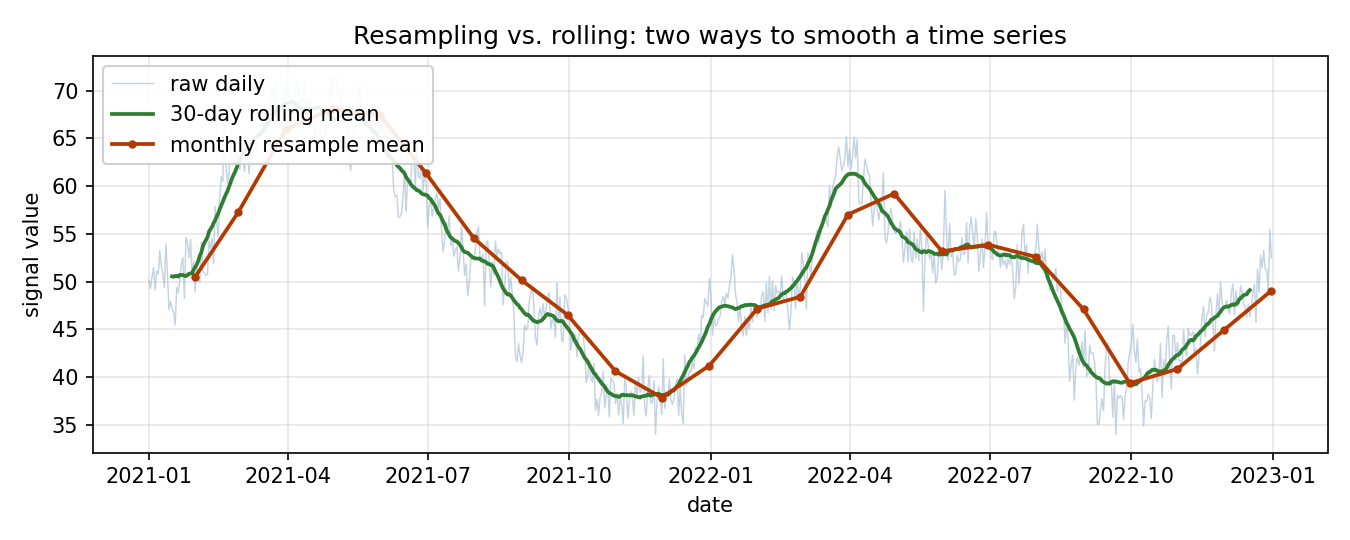
\includegraphics[width=\linewidth]{ts_resample.png}
\caption{Two ways to smooth. The pale line is the raw daily series. The orange markers are the monthly \code{resample('M').mean()} --- one point per month, sitting at month-end, a sparse summary. The green curve is the 30-day \code{rolling().mean()} --- a dense, continuous smoother at the original daily frequency. Both reveal the drift-plus-season structure that the raw fuzz hides; \code{resample} gives you fewer, calendar-aligned points, while \code{rolling} gives you a full-resolution trend line.}
\end{figure}

\subsection{When to reach for which}

The three tools answer different questions, and a quick decision rule keeps them straight. Ask \emph{what the output should look like}:

\begin{center}
\renewcommand{\arraystretch}{1.3}
\begin{tabular}{l l l}
\toprule
\textbf{You want\dots} & \textbf{Tool} & \textbf{Output frequency} \\
\midrule
fewer points, one summary per bin & \code{resample(f).agg} & coarser than input \\
the same value on a new grid       & \code{asfreq(f)}       & finer or coarser (no aggregation) \\
a smooth trend at full resolution  & \code{rolling(w).agg} & same as input \\
\bottomrule
\end{tabular}
\end{center}

A useful sanity check: \code{resample} and \code{asfreq} \emph{change the number of rows} (the index frequency changes); \code{rolling} \emph{preserves} it (only the values change, smoothed in place). If a smoothing step unexpectedly shrank your frame, you reached for the wrong one.

\begin{pyrefresh}
A rolling mean is a discrete \emph{convolution} of the series with a uniform window of weights $1/w$. That framing tells you why the edges are special: near the start and end there are fewer than $w$ neighbours, so by default those positions come back as \code{NaN} (pass \code{min\_periods} to relax this). It also hints at the richer cousins you will meet later: \code{.ewm()} (exponentially weighted, so recent points count more) and windowed \code{.corr()}/\code{.cov()} for moving relationships between two series.
\end{pyrefresh}

\section*{Section recap}
\addcontentsline{toc}{section}{Section recap}
\begin{itemize}
  \item Python's time stack: \code{datetime}/\code{dateutil} (flexible, slow, object arrays) and NumPy \code{datetime64} (fast, typed, rigid). Pandas fuses them as \code{Timestamp} $+$ \code{DatetimeIndex}.
  \item Three kinds of time data: \textbf{stamps} (\code{Timestamp}/\code{DatetimeIndex}, a point), \textbf{periods} (\code{Period}/\code{PeriodIndex}, a fixed-frequency bin), \textbf{durations} (\code{Timedelta}/\code{TimedeltaIndex}, a length). Stamp $-$ stamp $=$ duration.
  \item Build with \code{pd.to\_datetime} (flexible parsing; watch day/month ambiguity) and \code{date\_range}/\code{period\_range}/\code{timedelta\_range}. Frequency codes scale with a number (\code{'2D'}) and concatenate (\code{'2H30T'}); \code{MS}/\code{QS}/\code{YS} anchor at the start, bare \code{M}/\code{Q}/\code{A} at the end.
  \item A \code{DatetimeIndex} enables partial-string indexing: \code{data['2021']}, \code{data['2021-07']}, and inclusive date-range slices.
  \item \code{resample} $=$ groupby-over-time-bins reduction (down-sampling); \code{asfreq} $=$ point selection onto a new grid (up-sampling needs \code{ffill}/\code{bfill}).
  \item \code{.rolling(window)} smooths at the original frequency by sliding a window; use \code{center=True} to avoid lag.
\end{itemize}

\end{document}
